\section{Development of the trigger for \BdToKstmm}
\label{sec:lhcb:trigdev}

\subsection{Introduction}

The development of a new \lhcb trigger for 2011 was motivated by the significant change in the operating conditions of
both the \lhc and \lhcb between the 2010 and 2011 running periods. 
With the successful operation of the detector at the design luminosity in 2010, the decision was taken  
to go beyond this to counteract the reduced beam energy and number of proton bunches.
This was in order to acquire enough integrated luminosity for the \lhcb measurements of key channels, 
such as \Bsmm and \BdToKstmm~\cite{Adeva:2009ny}, to remain competitive with \cms in 2011.
This increase in the luminosity required the redevelopment of the trigger in order to keep 
a high efficiency for the main signal channels, chosen to represent the physics programme of \lhcb, whilst keeping 
the rate of background events taken at a reasonable level.

The design of the \lhcb trigger in 2010 contained an inclusive topological trigger~\cite{Alves:2008zz} which was designed to
 select hadronic \B decays, as well as several exclusive trigger algorithms to select particular decays such as \BdToKstmm.
The exclusive trigger algorithms were unworkable for the expected conditions for 2011 running due to the time taken to process an event in the trigger and 
the rate at which the exclusive trigger lines accepted background events.% in the 2010 periods where the \lhc tested the 2011 configuration.
The development of a muonic inclusive trigger was proposed since this was advantageous for both electroweak penguin decays 
such as \BdToKstmm and semi-leptonic decays such as $\B\to\D\mu\nu$.

The requirements for a new inclusive trigger in \lhcb were defined so that the new trigger should reject sufficient background events, keep a good enough signal efficiency
when compared to the previous exclusive triggers and minimise the acceptance effect for the distribution of the signal decays.
The rejection rate is correlated to the bandwidth in the trigger allowed for the trigger line.
The new inclusive trigger would be allocated 200\hz of bandwidth out of a total of 500\hz available for the topological triggers,
corresponding to a background rate of around 0.2\% when running at an average number of interactions per bunch crossing of $\mu=2.5$.

The hadronic topological trigger is an inclusive trigger which selects a 2, 3 or 4-track potential `\B' candidate by requiring candidates to have kinematic properties common to \B decays. 
They include the invariant mass,  momentum,  transverse momentum and the daughter track impact parameter.
The electroweak penguin decays, such as \BdToKstmm and \BsToPhimm, have two muons and two hadrons in their final state.
The high momentum requirements of muons to pass the \lhcb reconstruction mean that, on average, in the final state there are higher momentum muons then hadrons.
The semi-leptonic \B decays such as $\Bd\to\D^{(*)}\mu\nu$ have similar kinematics but the hadrons which come from a 
intermediate \D meson have a longer lifetime.
This allows the trigger to have  stricter requirements on the muon but needs looser requirements on the quality of the \B vertex 
and on the invariant mass of the $n$-body candidate as at least one of the daughter particles is missing.
%The trigger lines selecting these final states were called the \muntrack lines, divided up into the individual \muonetrack, \mutwotrack and \muthreetrack lines.

Simultaneously, a multi-variate topological trigger (\hlttwotopo) was also developed~\cite{Williams:1323557,Gligorov:1384380} 
using a Boosted Decision Tree (BDT)~\cite{Breiman,Roe,AdaBoost}.
In order to allow a BDT to select generic \bquark-hadron events in the trigger, the input variables were discretised to reduce 
 the dependence of the trigger efficiency on the data used to train the BDT.
%This discretisation of the input variables leads to the description of this MVA as a Bonsai Boosted Decision Tree (BBDT).
A muon-specific version of the BDT trigger was developed in parallel to the \muntrack lines, called the \mutopo trigger lines.
This ran a similarly trained BDT but with the added benefit of including information about the muon candidate in the $n$-body combination.

In order to develop a trigger line for analysis of general \B decays, consideration must be given to the distribution of events which pass the trigger.
The angular analysis of \BdToKstmm is sensitive to the acceptance effect caused by event reconstruction and selection~\cite{Blake:1322186,Serra:1239143}.
Measurements of the semi-leptonic decays requires a relatively unbiased lifetime and are hindered by cuts which have a non-trivial lifetime acceptance for the \D mesons.
The data used to develop the trigger for muonic \B decays are detailed in Section~\ref{sec:trigdev:data} and the resultant trigger configuration is given in Section~\ref{sec:trigdev:config}.
The results on testing the trigger on simulation and background data are shown in Section~\ref{sec:trigdev:results}.

\subsection{Datasets}
\label{sec:trigdev:data}

The datasets used in the optimisation of the trigger consist of samples of simulated data to represent the signal decays
and a sample of data events recorded to represent the expected background events.
The signal sample for \BdToKstmm consists of two sets of simulated events which have passed the \lhcb reconstruction. 
The first set has the expected offline selection applied and the second set contains events with extreme values of \ctl. 
These the events are particularly difficult to select since the extreme value of \ctl implies one low-momentum (soft) muon.
These extreme \ctl events also give maximum sensitivity to a measurement of \AFB.
 The conditions of the simulation used are the configuration available at the end of 2010 (MC10). 
The \ctl and \qsq distributions of this sample are shown in Fig.~\ref{fig:trigdev:kstmm}.
\begin{figure}[tbp]
\centering
\subfigure[]{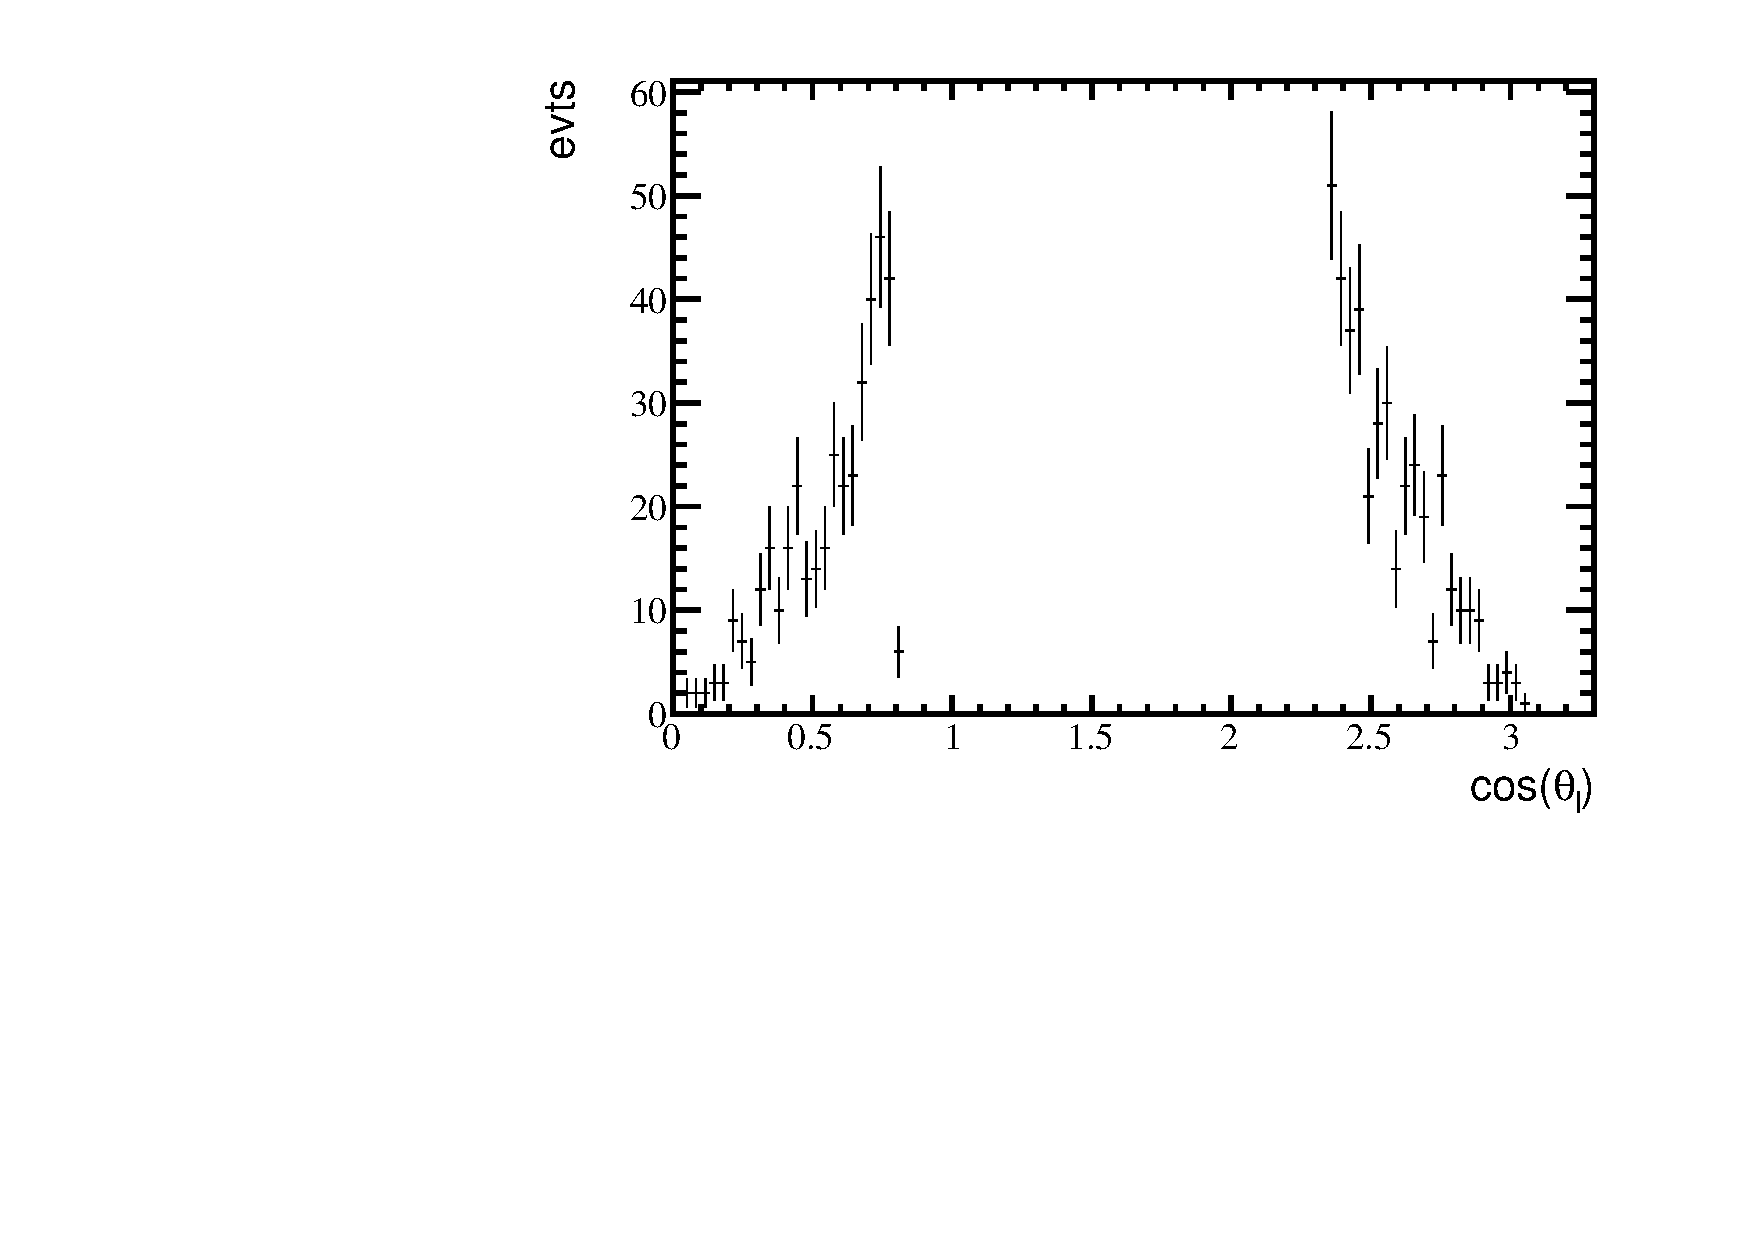
\includegraphics[width=0.48\columnwidth]{chapter3/figs/triggerdev/costhetal.pdf}}
\subfigure[]{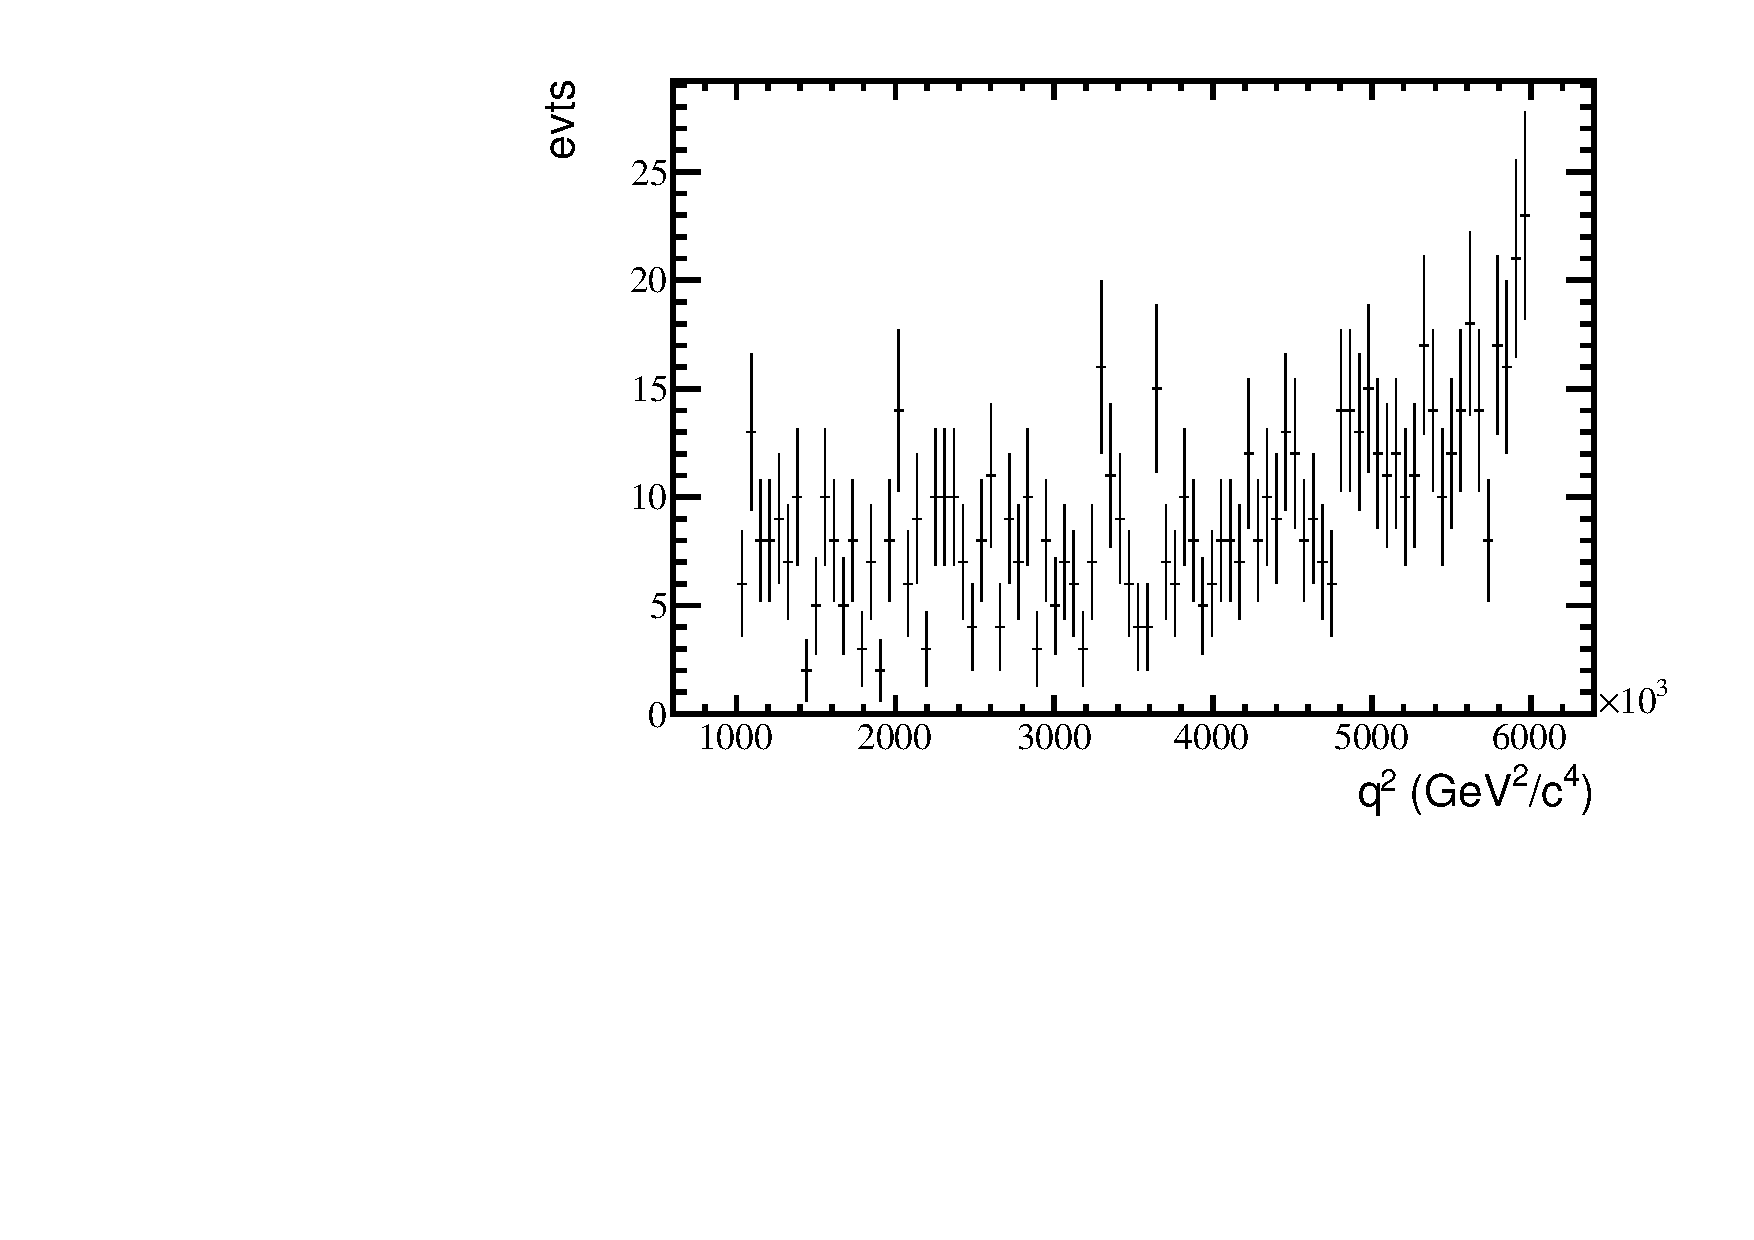
\includegraphics[width=0.48\columnwidth]{chapter3/figs/triggerdev/qsquare.pdf}}
\caption[\BdToKstmm simulated events used to optimise the trigger.]
{ The (a) \ctl and (b) \qsq distribution of the selected \BdToKstmm simulated events used to optimise the trigger efficiency. These events are the most sensitive 
to acceptance effects and hence provided a ideal sample to optimise against.~\label{fig:trigdev:kstmm} }
\end{figure}

Two signal samples were used to evaluate the efficiency of the trigger on semi-leptonic \B decays. 
These were one sample of \BtoDmunu simulated events and one sample of \BtoDsmunu simulated events.
These samples were generated using the latest conditions known before the start of data-taking, in the configuration MC09.
Other samples of selected simulated events for \BsToPhimm and $\Bs\to\jpsi\phi$ were provided to test and ensure that the trigger
was suitably inclusive.

The background data consisted of data events from a preparatory run of the \lhc in 2010 which was expected to be representative of the 
conditions for the 2011 data-taking period. 
This run has an average number of 2 interactions per bunch crossing and all the events in the data
 pass the \lzero trigger and the \hltone trigger, giving data which is representative of the type of events expected to be input to \hlttwo.

\subsection{Trigger configuration}
\label{sec:trigdev:config}

The trigger lines were written to minimise the time taken to process the event and the time taken to make a decision.
The first algorithmic optimisation was to compare all of the tracks used in \hlttwo with the track(s) that passed the \hltone trigger lines.
Tracks in \hlttwo are filtered based on whether both the tracks match, i.e they were created from the same hits in the tracking system.
This ensures consistency between the trigger lines and excludes mis-matched tracks.
The second stage is to make up-front cuts on the properties of the tracks to reduce the combinatorics to make the candidates.
A last algorithmic choice was to only form ($n+1$)-body candidates from candidates that pass the $n$-body criteria.
This means that 3(4)-body candidates are made from permissible 2(3) track combinations with an extra track added ensuring
that the number of candidates tested is minimised.

The number of different requirements and different priorities along with the time constraints of the trigger development lead to manual optimisation of the kinematic cuts in the \muntrack trigger.
Firstly, a basic set of cuts was identified that reduced the background rate to a sufficiently small level.
Secondly, additional cuts were introduced to maximise the signal efficiency on electroweak penguin and semi-leptonic decays.
Lastly, the full range of cuts were adjusted to minimise the acceptance effect on the \BdToKstmm signal decay.
Each of the kinematic quantities used to optimise the trigger selection are discussed below.
\begin{itemize}
\item The minimum \pt of the tracks was required to be over 600\mev and the minimum \pt of the muons was required to be above 800\mev.
The higher \pt requirement for the muons was based on the average kinematics for the the signal decays.
% This is 100 \mev above the minimum background required for the particles to be reconstructible in the trigger.
This was minimised to reduce any angular acceptance effect on \BdToKstmm tracks.
\item The sum of the \pt of all of the particles is a measure which allows for a more flexible combination
 where one high \pt track can compensate for several low \pt tracks.
 This is advantageous in both electroweak penguin and  semi-leptonic \B decays where there is a distinct separation between
  the muon kinematics and the hadronic kinematics.
%\item The momentum of each particle was left the minimum momentum required to pass .
\item The invariant mass of each track combination was required to be above the mass of the \D mesons in order to ensure decays with a \bquark quark are selected.
\item The \trchisq parametrises the quality of the track fit to the hits in the tracking stations. 
For the reconstruction software used in 2011, a maximum \trchisq of 4 per degree of freedom was sufficient to remove the majority of ghosts and clone tracks.
\item The \fdchisq is defined by the difference in \chisq value of the primary vertex fit when the tracks of the candidate are added to it.
This is a good measure for discriminating between combinations consisting of prompt and non-prompt tracks.
\item The direction angle, ($\delta_{\mathrm{PV}}$), is defined by the angle between the track direction and the related primary vertex, is a good measure to determine whether
the tracks of interest originate from the expected primary vertex. 
The tracks from signal decays was found to mostly be below $10(15)\mrad$ for tracks with (without) muon identification.
This is because of the harder kinematics of muons as opposed to the hadrons.
\item The distance of closest approach (DOCA) between the direction vector of the track and the primary vertex is another good measure to separate signal 
and background events and is highly correlated with the direction angle. 
A limit of a  maximum distance of closest approach of 12\mm was set for all tracks to pass the trigger.
\item The \ipchisq is a similar quantity to the distance of closest approach and also encompasses the error information from the resolution on the primary vertex.
\item The corrected mass is a quantity which attempts to balance the \pt of the particles in the $n$-body candidate with the \pt measured between the primary and secondary vertex~\cite{Abe:1997sb}.
This correction to the $n$-body mass is needed as the n-body combination is predominately a subset of the 
daughters from the \B decay.% and in the case of semi-leptonic decays will always be a subset of the daughters.
\end{itemize}
A list of the cuts used in the each of the three \muntrack trigger lines are given in Table~\ref{tbl:trigger:cuts}.
\begin{table}
\centering
\caption{ The kinematic and topological cuts used in the \muntrack trigger lines. ~\label{tbl:trigger:cuts} }
\begin{tabular}{|c|c|c|c|}
\hline
Kinematic quantity & 2-body & 3-body & 4-body \\
\hline
$M_{corr}^{max} (\gev) $&$ 7 $&$ 7 $&$ 7 $\\
$M_{corr}^{min} (\gev) $&$ 0 $&$ 4 $&$ 4 $\\
$\sum\pt$ (\gev)&$ 2 $&$ 2 $&$ 2.6 $\\
max \pt (\gev) &$ 1.5 $&$  1.5 $&$ 1.5 $\\
track \pt (\mev)&$ 600  $&$ 600$&$ 600$\\
muon \pt (\mev)&$ 800  $&$ 800$&$ 800$\\
momentum (\gev)&$ 5 $&$ 5 $&$ 5 $\\
$m_{\mu+(1,2,3)tracks} (\gev)$&$2$&$3$&$4$\\
\ipchisq&$16$&$16$&$16$\\
\trchisq&$4$&$4$&$4$\\
\fdchisq&$36$&$36$&$36$\\
$\cos\delta_{\mathrm{PV}}$ (track) (\rad)&$15$&$15$&$15$\\
$\cos\delta_{\mathrm{PV}}$ ($\mu$) (\rad)&$10$&$10$&$10$\\
DOCA(\mm)&$0.12$&$0.12$&$0.12$\\
\hline
\end{tabular}
\end{table}


\subsection{Results and Discussion}
\label{sec:trigdev:results}

There were three performance measures used to test the quality of the new trigger lines.
These are the signal efficiency, the expected rate of background rejection 
and the time taken to run the trigger lines.
%The timing of all of the lines were within the requirements of 20\ms. 
%Use was made of both pre-built tracks to minimise reconstruction within the \hlttwo algorithms themselves 
%and also selection criteria on each of the tracks independently before doing the combinatorics in order to minimise 
%the time spent calculating properties of $n$-body combinations that will be rejected.
The order within which each of the cuts were applied was also adjusted to minimise the time spent on the 
quantities which require the calculation of both a primary 
vertex and a secondary vertex compared to simple kinematic cuts.
The \hlttwo forward tracking was timed to take a total of 44\ms. On top of this, the \muonetrack line took 15\ms, the \mutwotrack line took 0.12\ms and the \muthreetrack line took a further 0.07\ms.
These timings are well within the limit of 20\ms limit for these lines.

A break down of the results for the different \muntrack lines is given in Table~\ref{tbl:triggereff}.
\begin{table}[tbp]
\centering
\caption[Trigger efficiencies of the \muntrack and \mutopo lines.]
{The trigger efficiency of selected simulated signal samples and of background data for the final configuration
of the \muonetrack and \mutwotrack lines along with the \mutopo lines and full \hlttwo trigger. ~\label{tbl:triggereff} }
\begin{tabular}{|c|c|c|c|c|}
\hline
Sample & \hlttwotopo  & \muntrack & \mutopo & \hlttwo \\
\hline
Selected K*\mumu & 79.8 \% &  79.6 \% &  79.3 \% &  92.9 \% \\
Reconstructible K*\mumu & 55.9 \% &  57.3 \% &  54.3 \% &  85.5 \% \\
$\D\mu\nu$  & 65.9 \% &  64.3 \% &  67.6 \% &  84.3 \% \\
$\phi\mumu$ &  76.1 \% &  80.0 \% &  75.9 \% &  95.1 \% \\	
 Background (train) &  0.9 \% &  0.47 \% &  0.27 \% &  5.2 \% \\
 Background (test) &  0.8 \% &  0.57 \% &  0.27 \% &  5.1 \% \\
\hline
\end{tabular}
\end{table}
The efficiency of each of the trigger lines in development per line on the two main signal samples along with the background rate is given in Table~\ref{tbl:trigeff:byline}.
\begin{table}
\centering
\caption{ The breakdown of trigger efficiency by line on \BdToKstmm, semi-leptonic and the background rejection rate. ~\label{tbl:trigeff:byline} }
\begin{tabular}{|c|c|c|c|}
\hline
Line & \BdToKstmm & \BtoDmunu  & Background Rate \\
\hline
%\hlttwotopo 2 Body & 60 \% &  39 \% &  0.3 \% \\
%\hlttwotopo 3 Body &  61 \% &  45 \% &  0.3 \% \\
%\hlttwotopo 4 Body &  38 \% &  18 \% &  0.3 \% \\
\mutopo 2 Body &  71 \% &  52 \% &  0.3 \% \\
\mutopo 3 Body &  69\% &  56 \% &  0.1 \% \\
\mutopo 4 Body &  42\% &  21 \% &  0.1 \% \\
\muntrack 1 &  73 \% &  47 \% &  0.3 \% \\
\muntrack 2 &  64 \% &  62 \% &  0.3 \% \\
\hline
All \mutopo & 79.3 \% &67.6 \% & 0.27 \% \\
All \muntrack & 79.6 \%& 67.3 \% & 0.47 \% \\
\hline
\end{tabular}
\end{table}
The efficiency of the \muntrack lines is comparable to the \mutopo for the main decay \BdToKstmm but the \mutwotrack line is the most efficient trigger on the semi-leptonic signal sample.
However, the \muntrack lines select more background than the equivalent \mutopo lines.

The efficiency of each of the $n$-body combinations for the \muntrack trigger lines as a function of \ctl and \qsq for offline selected \BdToKstmm simulation
 are given in Fig~\ref{fig:trigdev:eff:muntrack}.
\begin{figure}[tbp]
\centering
\subfigure{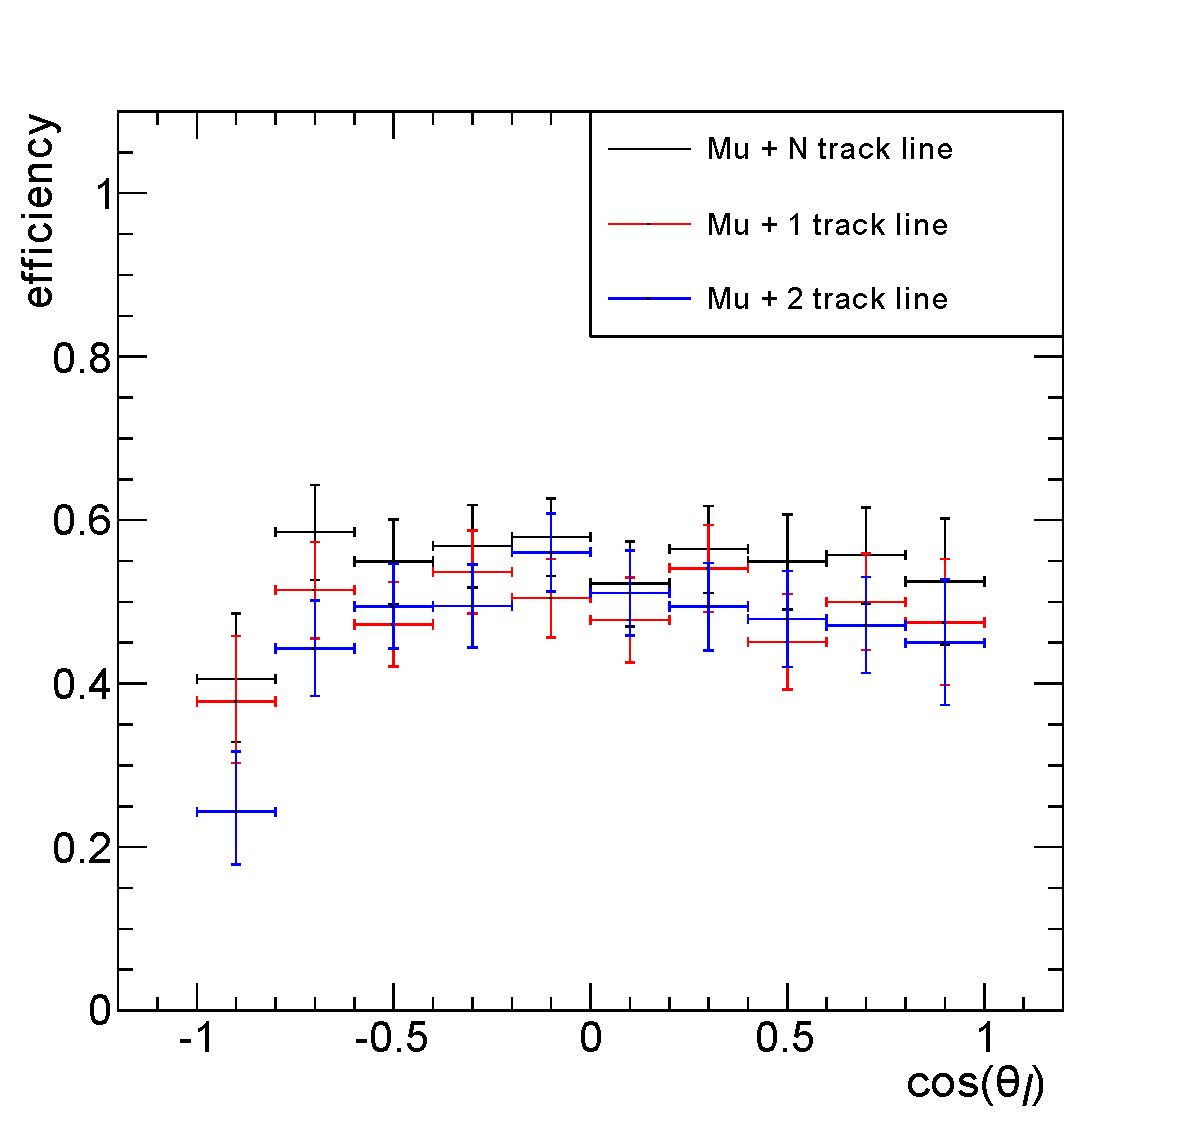
\includegraphics[width=0.48\columnwidth]{chapter3/figs/triggerdev/TrigEffMuNTrackLines_ThetaL_edit.pdf}}
\subfigure{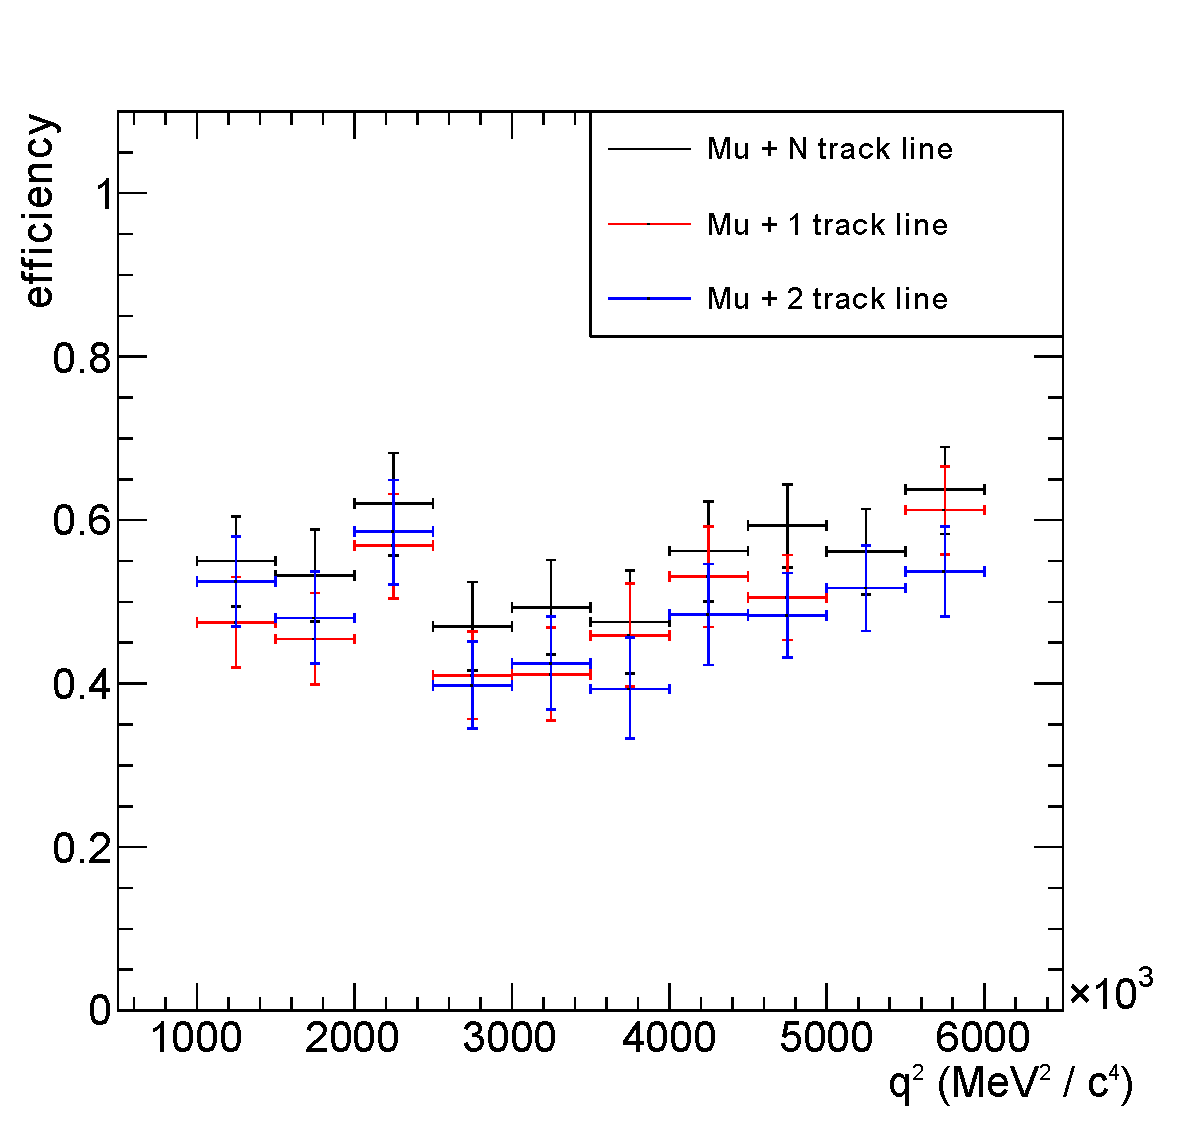
\includegraphics[width=0.48\columnwidth]{chapter3/figs/triggerdev/TrigEffMuNTrackLines_Qsquare.pdf}}
\caption[Efficiency of the \muntrack triggers on \BdToKstmm simulation.]
{ The \ctl and \qsq efficiency of the each individual \muntrack line. There is a slight bias in \ctl but not significant effects in \qsq. 
The drop in efficiency at low \ctl is also due to the low numbers of simulated statistics in that region. ~\label{fig:trigdev:eff:muntrack} }
\end{figure}
It is possible to see that there is no dramatic acceptance effect in \qsq but a slight bias in the lower region of \ctl.
The total efficiency of the \muntrack and the \hlttwotopo lines is shown in Fig~\ref{fig:trigdev:eff:comp}.
\begin{figure}[tbp]
\centering
\subfigure{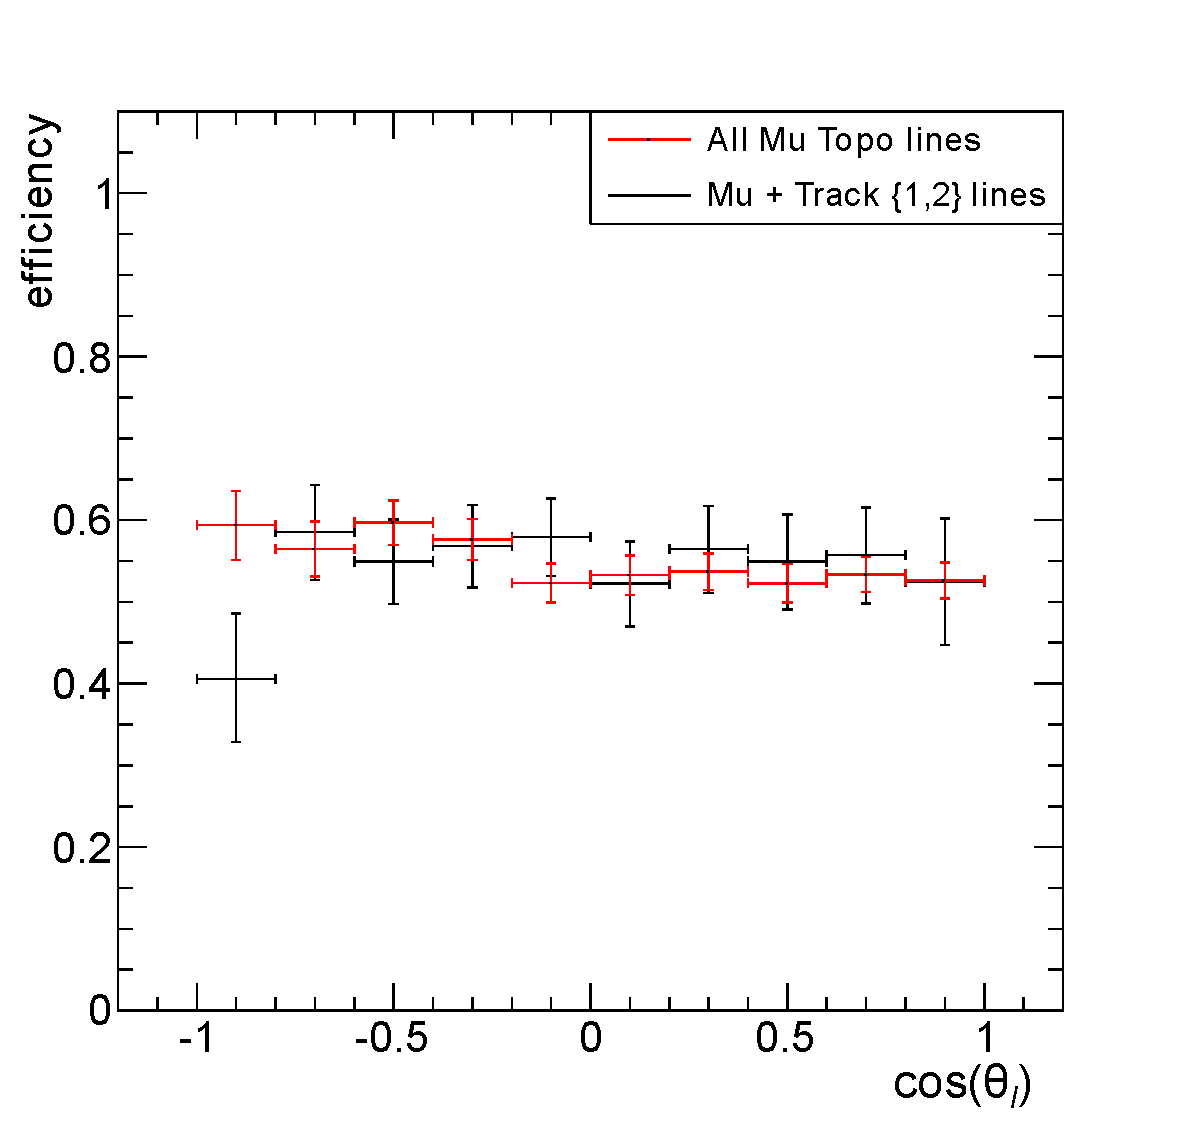
\includegraphics[width=0.48\columnwidth]{chapter3/figs/triggerdev/TrigEffCompareLines_ThetaL.pdf}}
\subfigure{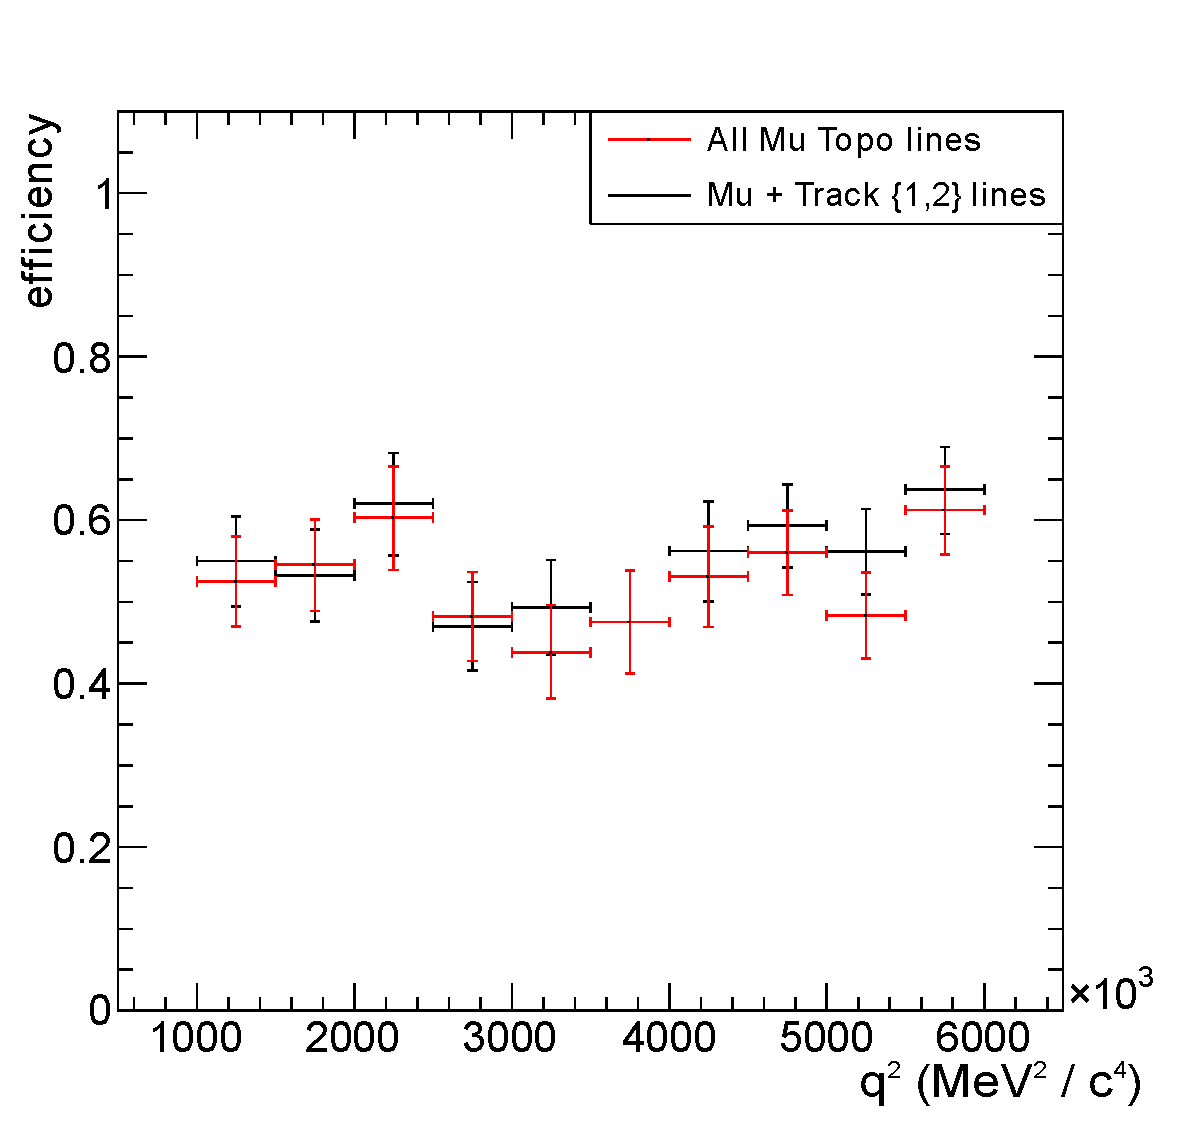
\includegraphics[width=0.48\columnwidth]{chapter3/figs/triggerdev/TrigEffCompareLines_Qsquare_edit.pdf}}
\caption[Comparison of the trigger line efficiency on \BdToKstmm.]
{ A comparison of the efficiency as a function of \ctl and \qsq efficiency of the \muntrack and the \hlttwotopo lines. ~\label{fig:trigdev:eff:comp} }
\end{figure}
The \hlttwotopo containing the muon-specific \mutopo has a comparable efficiency on simulated \BdToKstmm with a better acceptance effect in \ctl.
The improved performance of the \hlttwotopo when compared to the \muntrack lines comes from the gain in performance when using a multi-variate algorithm.
This allows advantage to be taken of correlations between the kinematic variables for each of the daughters and of the $n$-body track combinations.




